% Original research-seminar simulation. ALL measurements and maps are synthetic.
\documentclass[11pt,aspectratio=169]{beamer}
\usetheme{AnnArbor}
\usecolortheme{spruce}
\usepackage{amsmath,booktabs,graphicx,subcaption,pgfplots}
\pgfplotsset{compat=1.18}
\graphicspath{{assets/}}
\setbeamertemplate{navigation symbols}{}
\title[River restoration]{Did restoration change the river?}
\subtitle{A before--after comparison with a control reach}
\author{Ecology methods seminar}
\institute{Synthetic field study}
\date{Study design 11}
\begin{document}
\begin{frame}[plain]\titlepage\end{frame}
\section{Field question}
\begin{frame}{A greener image is a hypothesis, not an effect estimate}
\begin{figure}
\centering
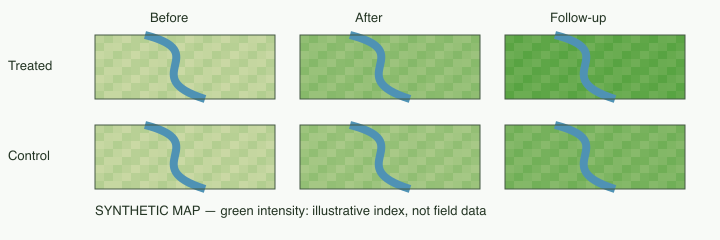
\includegraphics[width=.88\textwidth]{river-transects.png}
\caption{Invented sampling reaches. Colour encodes a synthetic vegetation index; no satellite or field observations are shown.}
\end{figure}
\end{frame}
\begin{frame}{Write the estimand before comparing means}
\begin{block}{Scientific question}
How much did the intervention change the treated reach's response relative to the change that would have occurred without it?
\end{block}
\begin{itemize}
\item Treatment unit: reach, not each pixel in an image.
\item Response: a prespecified index measured in comparable seasons.
\item Counterfactual: the treated reach without restoration is unobserved.
\end{itemize}
\end{frame}
\section{Design}
\begin{frame}{A control reach helps expose a shared seasonal change}
\begin{table}\centering
\begin{tabular}{lrrr}\toprule
Reach & Before & After & Change\\\midrule
Treated & 4.0 & 6.0 & $+2.0$\\
Control & 3.5 & 4.5 & $+1.0$\\\bottomrule
\end{tabular}
\caption{Synthetic index values in arbitrary units; illustrative means only.}
\end{table}
\pause
\[
 \widehat\delta=(6.0-4.0)-(4.5-3.5)=1.0.
\]
The before--after treated change is not the same estimand as this contrast.
\end{frame}
\begin{frame}{Put the identifying assumption in ordinary language}
\begin{alertblock}{Parallel untreated changes}
Without restoration, the treated reach would have changed by the same amount as the control reach over this interval.
\end{alertblock}
\begin{enumerate}
\item Check earlier trends when observations exist.
\item Investigate disturbances affecting only one reach.
\item Consider whether restoration changes the control reach too.
\end{enumerate}
\end{frame}
\section{Evidence}
\begin{frame}{Show variability alongside the mean contrast}
\begin{columns}[T]
\begin{column}{.6\textwidth}
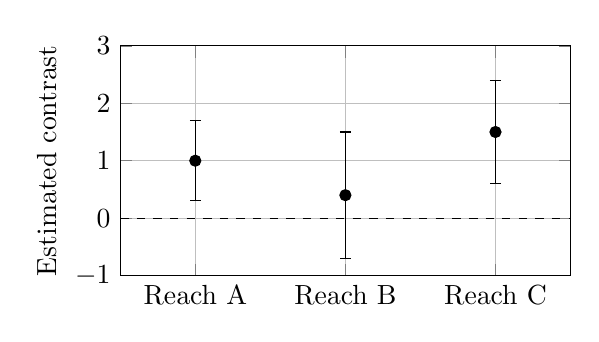
\begin{tikzpicture}\begin{axis}[width=7.3cm,height=4.5cm,xmin=.5,xmax=3.5,ymin=-1,ymax=3,
 xtick={1,2,3},xticklabels={Reach A,Reach B,Reach C},ylabel={Estimated contrast},grid=major]
\addplot[only marks,mark=*,error bars/.cd,y dir=both,y explicit] coordinates {(1,1) +- (0,.7) (2,.4) +- (0,1.1) (3,1.5) +- (0,.9)};
\addplot[dashed,domain=.5:3.5] {0};
\end{axis}\end{tikzpicture}
\end{column}
\begin{column}{.36\textwidth}
\small Synthetic estimates and illustrative intervals. Their widths are chosen for discussion, not computed from a field dataset.
\medskip
Which differences reflect evidence, and which may reflect noisy sampling?
\end{column}
\end{columns}
\end{frame}
\begin{frame}{A crop can hide context}
\begin{figure}
\begin{subfigure}{.46\textwidth}\centering
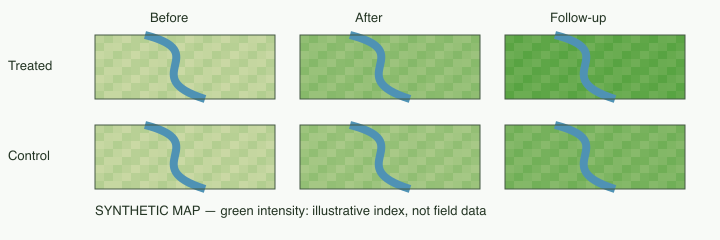
\includegraphics[width=\linewidth]{river-transects.png}
\caption{The full synthetic sampling map.}
\end{subfigure}\hfill
\begin{subfigure}{.46\textwidth}\centering
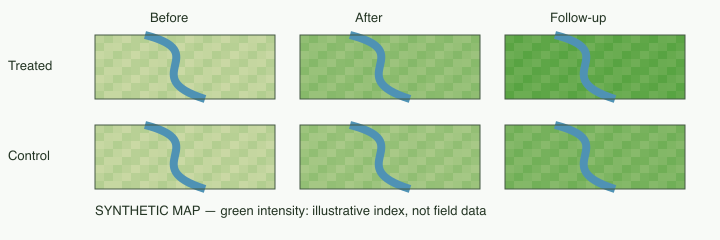
\includegraphics[width=\linewidth,trim=360 0 0 0,clip]{river-transects.png}
\caption{A deliberately cropped view.}
\end{subfigure}
\caption{Image selection is a reporting decision. State the spatial support of every summary.}
\end{figure}
\end{frame}
\section{Interpretation}
\begin{frame}{What the study can and cannot support}
\begin{columns}[T]
\begin{column}{.48\textwidth}\begin{exampleblock}{Supported description}
In the invented data, the treated mean rises more than the control mean.
\end{exampleblock}\end{column}
\begin{column}{.48\textwidth}\begin{alertblock}{Conditional interpretation}
A causal claim additionally needs the untreated-trend assumption, comparable measurement and no relevant spillover.
\end{alertblock}\end{column}
\end{columns}
\note{Ask whether hundreds of pixels create hundreds of independent treatment assignments. They do not.}
\end{frame}
\begin{frame}{The next field season should reduce one uncertainty}
\begin{enumerate}
\item Add comparable pre-intervention observations.
\item Replicate treatment at the reach level where feasible.
\item Prespecify seasonal sampling and missing-data rules.
\item Report both spatial heterogeneity and the aggregate contrast.
\end{enumerate}
\bigskip
\textbf{Seminar question:} which additional measurement would most change your interpretation?
\end{frame}
\appendix
\begin{frame}{Data provenance and reuse}
\small
All numbers, intervals and imagery in this deck were generated for renderer testing. No ecological site, intervention, research team or published study is being described.
\medskip
The asset is checked in beside the sources. Its deterministic generator and the values used in the figures are documented in the fixture README, so the deck compiles without network access or private files.
\end{frame}
\end{document}
